\section{Special relativity}
\paragraph{Motivation} Lack of agreement between Newton's laws and electromagnetic theory (Maxwell equations)

\paragraph{Example of disagreement}
Given this system:
\begin{center}
	\includegraphics[width=\linewidth]{./lect20/pic1.png}
\end{center}

This is what sees observer in resting frame of reference. The observer in fast moving system sees something else. Since system is moving it can be described as current and there is new force (magnetic) downwards: 


\begin{center}
	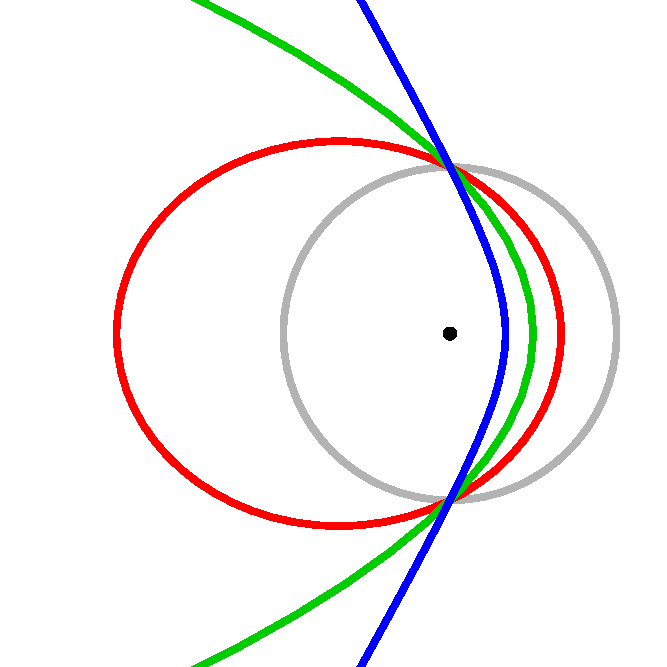
\includegraphics[width=\linewidth]{./lect20/pic2.png}
\end{center}

\subparagraph{Solution of special relativity}
The system is still in equilibrium, since $F_E$ grows since density of electrical charge in a rod grows because of Lorentz contraction.

\paragraph{Michelson-Morley experiment} is another example of problem. Special relativity explains there is no ether.

\paragraph{Notes on known in 1904}
\begin{itemize}
	\item Electromagnetic radiation is moving at speed of light
	\item Speed of light is finite. It was first measured in 1676.
\end{itemize}

\subsection{Assumption of special relativity}
\begin{itemize}
	\item Speed of light in vacuum is constant and denoted $c$.
	\item Symmetry. Our space is isotropic and homogeneous. The laws of physics are invariant (i.e. identical) in all inertial systems (non-accelerating frames of reference).
\end{itemize}

\paragraph{Experiment 1}


\begin{center}
	\includegraphics[width=\linewidth]{./lect20/pic3.png}
\end{center}

Time that takes light to get to the mirror and back is $t^\prime = \frac{L_0}{c}$. Then train passes $vt^\prime$ until it light gets to the mirror. And since speed of light is constant, light passes $ct^\prime$.
\begin{center}
	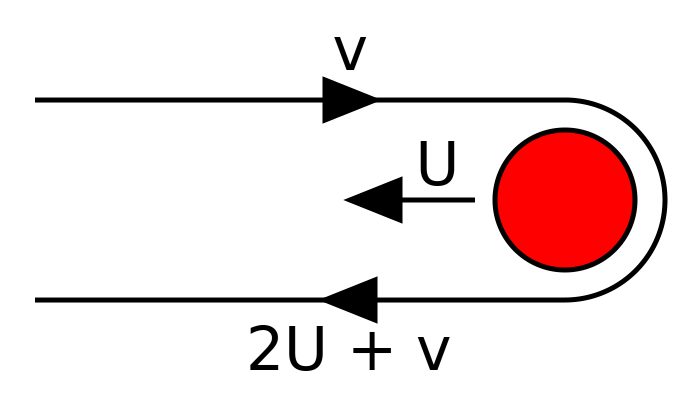
\includegraphics[width=\linewidth]{./lect20/pic4.png}
\end{center}

We get the following:

$$\left(vt^\prime\right)^2 + L_0^2 = \left(ct^\prime\right)^2$$
$${t^\prime}^2 \left(c^2 - v^2\right) = L_0^2$$
$$t^\prime = \frac{L_0}{\sqrt{c^2-v^2}} = \frac{\frac{L_0}{c}}{sqrt{1-\frac{v^2}{c^2}}}$$

Since $\frac{L_0}{c} = t_0$:
$$t^\prime = \frac{L_0}{\sqrt{c^2-v^2}} = \frac{t_0}{sqrt{1-\frac{v^2}{c^2}}}$$

Define $\gamma = \frac{1}{sqrt{1-\frac{v^2}{c^2}}} \geq 1$.


Observer in train used single clock. Single clock to measure difference between two events is proper time. Event is a point in four-dimensional space: $\left( x,y,z,w \right)$. 

Proper time is the shortest time between two events.

\subsection{Lorentz transformation}
For two frame of reference that synchronized their clock at $t=t^\prime=0$ when they are at same place:


\begin{center}
	\includegraphics[scale=0.20]{./lect20/pic5.png}
\end{center}

In frame of reference $S^\prime$. At $t^\prime=0$ a frame $S^\prime$ turns on light which is spread as ${x^\prime}^2 + {y^\prime}^2 + {z^\prime}^2 = \left(ct^\prime\right)^2$.

For stationary frame of reference, $x^2+y^2+z^2= \left(ct\right)^2$, since speed of light is constant. By substituting Galileo transformation $x^\prime  =x - vt$ we get wrong equation: $x^2 -2xvt + y^2 + z^2  = \left(ct\right)^2$ (inconsistent with what we got from constant speed of light).


\paragraph{Define new transformation} It should be:

\begin{itemize}
	\item linear (to have inverse transformation). General form is $$\begin{cases*}
		x^\prime = \alpha x + \epsilon t\\
	y^\prime = y\\
	z^\prime = z\\
	t^\prime = \lambda x - \eta t\\
	\end{cases*}$$
	\item $y^\prime = y$ and $z^\prime = z$ due to symmetry.
	\item At low speed $\frac{v}{c} \ll 1$we get back to Newton-Galileo 
\end{itemize}

We can find $\alpha, \epsilon, \delta, \eta$ by substituting equations for $S$ and $S^\prime$:

$$\begin{cases*}
x^\prime = \frac{x-vt}{\sqrt{1-\frac{v^2}{c^2}}}\\
y^\prime = y\\
z^\prime = z\\
t^\prime = \frac{t-\frac{v}{c^2}x}{\sqrt{1-\frac{v^2}{c^2}}}\\
\end{cases*}$$

Define $$\beta = \frac{v}{c}$$ and $\gamma = \frac{1}{\sqrt{1-\beta^2}}$. Then

$$\begin{cases*}
x^\prime = \gamma \left(x-\beta ct\right)\\
y^\prime = y\\
z^\prime = z\\
t^\prime = \gamma \left( t - \frac{\beta x}{c} \right)\\
\end{cases*}$$

Inverse transformation is acquired by replacing $v$ with $-v$ (symmetry of observers)
$$\begin{cases*}
x = \gamma \left(x^\prime+\beta ct\right)\\
y = y^\prime\\
z = z^\prime\\
t = \gamma \left( t^\prime + \frac{\beta x^\prime}{c} \right)\\
\end{cases*}$$